\documentclass[11pt]{article}
\usepackage[a4paper,margin=2.5cm]{geometry}
\usepackage[T1]{fontenc}
\usepackage{lmodern,microtype,booktabs,graphicx,amsmath,siunitx,xcolor,hyperref,url}
\usepackage[numbers,sort&compress]{natbib}
\sisetup{group-separator={,},group-minimum-digits=4}
\graphicspath{{figures/}}
\title{Historical supporting results: AG-DATA forecast benchmark}
\author{}\date{}
\begin{document}\maketitle
\noindent This separate supporting document preserves analyses from commit \texttt{2a97a7e}. It is not the primary reproduced study. Original full-size execution and panel construction remain incompletely attributable; historical model choices, source-completeness comparisons, retraining, timing ablations and decision-rule backtests are exploratory supporting evidence. Older p values use dependence heuristics, not validated inferential guarantees. These results do not independently confirm LightGBM superiority or causal effects of missingness. Cross-references below are internal to this historical account; the primary paper supplies the current interpretation and limitations.
\section{Data and provenance audit}\label{sec:data}

\paragraph{Sources.}
Model development used an archive of AGMARKNET daily reports for 2001-01-10 to 2026-04-21: a Kaggle dataset (\texttt{khandelwalmanas/daily-commodity-prices-india}, version 134, GODL-India).
It has \num{75984017} rows; after quality classification and business-key de-duplication, \num{75644801} rows remain.
Its columns match the official data.gov.in resource \emph{Variety-wise Daily Market Prices Data of Commodity}.
After development, an API key became available. We back-filled \num{7720662} official records for 2025-10-01 to 2026-10-22, one request series per date, 387 dates with no failure.
Our second layer combines the archive before 2025-10-01 with the official record afterwards, for \num{82114083} rows in total.

\paragraph{Scope and panel.}
We use 36 staple commodities: vegetables, fruits, cereals, pulses, oilseeds and cotton.
They were chosen from training-period data:
\begin{enumerate}
  \item take an a-priori list of crop-name patterns;
  \item keep matches with more than \num{50000} valid reports in 2021--2023;
  \item drop two duplicate or processed forms;
  \item keep the 36 most-reported.
\end{enumerate}
An entity (series) is (state, district, market, commodity, variety).
It is in the panel if it has at least 300 report days in 2021--2023, which gives \num{11845} series and \num{21.06}M feature rows.
A causal sanity rule removes reports more than a factor of five from the geometric mean of the previous ten reports (\num{28567} reports, 0.086\%).

\paragraph{Identifier drift.}
Several changes in how identifiers are published would break series if left untreated:
\begin{itemize}
  \item many series switch their grade label from \emph{FAQ} to \emph{Local} in January 2025. No (state, district, market, commodity, variety, date) key carries two grades in the archive since 2023, so grade is an attribute. The official record is different: there, 1.2\% of entity-days (\num{85315}) carry several grades, and a deterministic rule keeps one of them;
  \item markets gain an `` APMC'' suffix with the AGMARKNET~2.0 portal (live 2025-11-07);
  \item the official API writes no space before ``('' and uses ``Keralam'' for Kerala.
\end{itemize}
One normalisation rule, shared by the batch and streaming paths, maps all of these. On 2026-04-20, all \num{5152} valid archive keys are found among the \num{22716} official records.

\paragraph{Mirror completeness.}
Table~\ref{tab:mirror} compares daily volumes.
On the sample days in Table~\ref{tab:mirror} the mirror holds 94--100\% of official reports before October 2025 and 0--54\% afterwards. By month, it holds 70.4\% in October 2025 and 5.9--38.9\% from November 2025 to April 2026, which is 30.0\% overall for 2025-10-01 to 2026-04-21.
Every mirror record in that window exists in the official data, and 99.33\% have an identical modal price. The mirror is incomplete, not corrupt.
Missing reports lengthen the gaps between consecutive reports of a series:
\begin{itemize}
  \item the median gap is 3 days in the mirror and 1 day in the official record;
  \item 16.2\% of mirror gaps exceed a week, against 2.4\% in the official record.
\end{itemize}
Longer gaps push ``next report'' targets further ahead and thin the trailing windows the features rely on.

\begin{table}[t]\centering\small
\caption{Daily report counts, official API versus the public mirror (sample days).}\label{tab:mirror}
\begin{tabular}{@{}lrrr@{}}\toprule
Date & Official & Mirror & Share\\\midrule
2025-03-12 & 22,040 & 21,967 & 0.997\\
2025-09-17 & 20,703 & 19,542 & 0.944\\
2025-10-15 & 21,899 & 20,611 & 0.941\\
2025-11-20 & 17,824 & 0 & 0.000\\
2025-12-17 & 19,566 & 10,559 & 0.540\\
2026-02-18 & 18,979 & 5,992 & 0.316\\
2026-04-20 & 22,716 & 5,162 & 0.227\\\bottomrule
\end{tabular}\end{table}

\section{Forecasting task and evaluation protocol}\label{sec:protocol}

\paragraph{Task.}
Entity $e$ reports modal prices $P_{e,t}$ (INR per quintal) on irregular dates.
For an origin $t$ and $h\in\{3,7,14\}$ days, the target is the first report dated in $[t+h,t+h+3]$. If there is none, there is no label.
The \emph{next} horizon is the next report, if it falls within 7 days.
Models predict $y=\ln P_{e,\tau}-\ln P_{e,t}$, and errors are measured in rupees on $P_{e,t}\exp(\hat y)$.

\paragraph{Periods (main experiment).}
\begin{itemize}
  \item Training origins: 2016--2023.
  \item Validation: 2024, used for tuning, model choice and conformal calibration.
  \item Test origins: 2025-01-01 to 2026-04-20, scored once.
\end{itemize}
A row is kept only if its target date also lies in its period; a unit test enforces this purge.
A perturbation test multiplies all future prices, and all other entities' prices, by arbitrary factors and requires every feature at the origin to be unchanged.
Training uses a uniform sample of $2\times10^6$ rows per horizon (fixed seed).

\paragraph{Selection.}
The family with the lowest validation MAE is selected, baselines included.
The search space was amended twice, both times on validation evidence, before any test metric was read:
\begin{itemize}
  \item first, after squared-loss learners tied persistence;
  \item second, after finding that MLlib's absolute-loss boosting is mis-scaled for log returns.
\end{itemize}
An aborted first run had already written test predictions for one horizon. They were deleted unread, and we disclose this.

\paragraph{Metrics and tests.}
We report:
\begin{itemize}
  \item MAE, RMSE, WAPE, sMAPE and bias;
  \item MASE, scaled by each entity's in-sample $h$-step naive MAE on training rows \cite{hyndman2006another};
  \item MAE relative to persistence on identical rows;
  \item the share of series (at least 30 test rows) on which a model beats persistence.
\end{itemize}
Diebold--Mariano tests \cite{diebold1995comparing} use daily mean absolute-error differences, a Newey--West variance with lag $h+3$ (7 for the next report) and the HLN correction. Same-day errors are aggregated first because they are correlated across markets.

\paragraph{Frozen-model and retraining evaluations.}
After the official back-fill, we score the frozen models, quantiles and MASE scales on complete official data:
\begin{itemize}
  \item on the original test period;
  \item on 2026-04-22 to 2026-10-22, reports first downloaded after the models were saved.
\end{itemize}
Separately, we retrain with the same search space, selection rule, sample size and seed, on a protocol fixed before the run:
\begin{itemize}
  \item training: 2016--2024;
  \item validation: 2025;
  \item final test: 2026-01-01 to 2026-10-22, not used for any retraining choice. Its first months overlap the main test, and its later months had already been used to score the frozen models.
\end{itemize}


\paragraph{Locked retrospective robustness protocol.}
A separate resource-limited sensitivity experiment uses 2024 training origins, January--June 2025 for selection and early stopping, July--December 2025 for interval calibration, and January--October 2026 for retrospective evaluation. Targets are purged at each period boundary. It compares the original cleaned features with a second pipeline retaining reports flagged by the fivefold jump rule; other validity checks and panel membership are preserved. The second pipeline begins in October 2022, providing over a year of history before training origins. This is not an exact reproduction of the original feature construction, whose source state is unproven.
Each regime trains on 500,000 deterministic hash-selected rows, tests 31 and 63 leaves with at most 800 boosting rounds and one fixed seed, and compares all five simple baselines on identical rows. MASE scales use all training-period rows. Calibration observations have no role in hyperparameter choice or early stopping. Calendar-day paired moving-block bootstrap intervals use 14- and 28-day blocks and 500 replicates; separate entity-cluster intervals describe between-series sensitivity, not joint two-way inference. Eight primary candidate--persistence tests (two regimes, four horizons) are corrected together using Holm. For these tests, calendar-day total loss differences divided by a constant target pooled row-weighted MAE; the older daily-mean tests target a different weighting. These changes do not retrospectively correct the original protocol.
The protocol, imported module paths, source commit, dependencies, split bounds and SHA256 hashes of inputs, models and saved predictions are recorded. Generated tables are checked against saved predictions. All 2026 outcomes were already available during study design, so this experiment measures retrospective robustness and cannot constitute independent confirmation.


\paragraph{Release reproduction and dependence sensitivity.}
The clean-source release rebuilds both cleaning regimes from the same silver data and fixed panel, rather than reusing either historical feature table. Source, silver/panel inputs, shard definitions and the assembled executable JAR are hashed before execution, verified unchanged around shard execution, and bound to output checksums, commands, runtime versions and exit codes. This is observed execution attestation, not an independent build witness. It reproduces the smaller study, not the full-size historical MLlib experiments or the original panel-construction process.
A subsequent automated methodological review found that daily loss dependence can extend beyond the original bandwidths. Block choice matters under dependent resampling \cite{politis2004block}; we therefore add explicitly retrospective sensitivities with all 28-, 42- and 56-day blocks, circular and non-circular, and 2,000 replicates each. We report asymptotic normal HAC diagnostics at those three bandwidths without a fixed-horizon HLN correction. The older helper coupled that horizon correction to the covariance bandwidth; for irregular report gaps its finite-sample justification is unestablished. Those historical p values are retained only as heuristic diagnostics. Holm corrections are separate across each declared eight-comparison bandwidth family, with no favourable bandwidth selected.
Inference is conditional on the fitted models and observed panel, and relies on an adequate weak-dependence and stationarity approximation. Same-day aggregation retains joint observed cross-market variation, but does not eliminate serial dependence or seasonality. Longer blocks preserve more dependence while leaving fewer temporal spans; more replicates improve Monte Carlo resolution, not sampling validity. The interval estimates have not been shown to attain nominal coverage. Entity resampling is exploratory sensitivity under correlated series, not a confidence guarantee for independent new markets. We report direct entity-ratio quantiles, subgroup errors, daily losses/counts, autocorrelation and MASE exclusions. A human expert statistical review remains outstanding.

\section{Methods}\label{sec:methods}

\paragraph{Features.}
Each origin carries 24 base features plus one horizon-specific seasonal feature, all computed from reports dated $\le t$ (Table~\ref{tab:features}).
Missing values are set to zero. Each feature that can be missing has an indicator or count, so no fitted imputation can leak.
The cross-market features use other markets' reports of the \emph{same day}, which assumes those are published by the end of day $t$.
We test this assumption with a variant that uses the previous day's cross-market values instead (Section~\ref{sec:point}).

\begin{table}[t]\centering\small
\caption{Feature groups ($\ell=\ln P$); all frames end at the origin.}\label{tab:features}
\begin{tabular}{@{}lp{0.74\linewidth}@{}}\toprule
Group & Features\\\midrule
Level and lags & $\ell_t$; differences to the 1st, 2nd and 5th previous reports; days since the previous report\\
Rolling (7/30/90 d) & deviation from the rolling mean; standard deviation (30, 90); report counts (30, 90); distance to the 30-day max and min\\
Range & $(\max-\min)/\text{modal}$ on day $t$\\
Seasonal & deviation from the level at $t-365\pm3$; availability indicator; last year's change from $t-365$ to $t+h-365$\\
Cross-market & same-day mean 30-day deviation and last return of the commodity, nationally and within the state; number of reporting markets\\
Calendar & day of year (sine, cosine); day of week\\
Categorical & commodity\\\bottomrule
\end{tabular}\end{table}

\paragraph{Baselines.}
\begin{itemize}
  \item Persistence ($\hat y=0$).
  \item Geometric moving averages over 7 and 30 days.
  \item Seasonal naive: last year's level around $t+h-365$, falling back to persistence when that is missing.
  \item Seasonal-adjusted persistence: today's level times last year's change over the same horizon.
  \item Per-series simple exponential smoothing (SES) on $\ell$, with the smoothing weight chosen per series on training origins.
  \item A global LightGBM model with an L1 objective, trained on the same features and training sample, tuned and early-stopped on validation only; predictions of three seeds are ensembled.
\end{itemize}

\paragraph{Learners.}
Each horizon has its own Spark MLlib model (direct strategy). The candidates are:
\begin{itemize}
  \item ridge and Huber regression on standardised features with one-hot commodity;
  \item a random forest (60 trees, depth 10);
  \item gradient-boosted trees with squared loss;
  \item gradient-boosted trees with absolute loss.
\end{itemize}
MLlib's absolute-loss boosting fits trees after the first to the sign of the residual, without a leaf line search, so each iteration moves predictions by up to the step size.
We therefore train these models on the target in percent, with step sizes of 0.25--0.5, and rescale inside the persisted pipeline. A unit test shows that this recovers the conditional median of a zero-inflated target.

\paragraph{Intervals.}
For the selected model, validation residuals are grouped into five bins by 30-day log-price volatility, with bin edges from validation quantiles.
Each bin's 5/10/90/95\% residual quantiles give 80\% and 90\% intervals.
Exchangeability does not hold for time series, so coverage is measured on test data \cite{gibbs2021adaptive}.

\section{Point-forecast results and evidence status}\label{sec:point}



\paragraph{Validation: the scoring function decides.}
On the 2024 validation tuning sample (\num{600000} rows) at the next-report horizon, persistence has an MAE of 210.7 rupees per quintal. The squared-loss learners do not beat it:
\begin{itemize}
  \item ridge regression: 228.1;
  \item squared-loss boosting: 214.8;
  \item the random forest: 211.1, a tie with persistence;
  \item Huber regression: 212.5.
\end{itemize}
Absolute-loss boosting reaches 205.3.
At 7 and 14 days, every learner beats persistence on validation, and the random forest is selected.
This is the pattern that elicitation theory predicts when a large share of the targets is exactly zero \cite{gneiting2011making}. The conditional median of the change is then often zero, while the conditional mean is not.

\paragraph{Historical main test (execution state incompletely attributable).}
Table~\ref{tab:main} reports the selected models on 1.55--1.67 million test forecasts per horizon.
Their MAE is 2.9--7.7\% below persistence, under the historical specification. Its small test p values are conditional on an incompletely verified execution state and on the dependence assumptions discussed in Section~\ref{sec:discussion}.
On test data the random forest does not beat persistence at the next report either (DM $p=0.28$).
All other baselines are worse than persistence at every horizon:
\begin{itemize}
  \item moving averages: relative MAE 1.005--1.795;
  \item seasonal naive: 2.50--5.11;
  \item seasonal-adjusted persistence: 1.10--1.34.
\end{itemize}
The improvement is broad. The selected model beats persistence on 58.5\%, 68.8\%, 75.0\% and 76.4\% of series with at least 30 test rows.

\begin{table}[t]\centering\small
\caption{Historical main test, 2025-01-01 to 2026-04-20 (mirror data). The relative MAE is the model's MAE divided by that of persistence on identical rows. DM: Diebold--Mariano test against persistence.}\label{tab:main}
\begin{tabular}{@{}lrrrrrr@{}}\toprule
Horizon & Persistence MAE & Selected & MAE & Rel.\ MAE & DM $p$ & Series better\\\midrule
next & 189.0 & GBT, abs.\ loss & 183.5 & 0.971 & $1\times10^{-22}$ & 58.5\%\\
3 d & 242.6 & GBT, abs.\ loss & 231.1 & 0.953 & $4\times10^{-47}$ & 68.8\%\\
7 d & 308.8 & random forest & 289.7 & 0.938 & $4\times10^{-39}$ & 75.0\%\\
14 d & 397.0 & random forest & 366.4 & 0.923 & $9\times10^{-29}$ & 76.4\%\\\bottomrule
\end{tabular}\end{table}

\paragraph{Scaled errors disagree.}
Averaged over rows, MASE does not favour the learned models everywhere:
\begin{itemize}
  \item next report: 1.559 for the selected model against 1.520 for persistence;
  \item 7 days: 1.430 against 1.257;
  \item 3 days: 1.680 against 1.716;
  \item 14 days: 1.056 against 1.113.
\end{itemize}
The rupee gains therefore come mainly from series and days with large absolute price moves. On rows that are small relative to the series' own naive error, the models are no better than persistence and sometimes worse.
We report both measures, because they answer different questions: aggregate rupee error, and an equal-weighted error per row.

\paragraph{Stronger and simpler baselines.}
Two further baselines bracket the MLlib model.
\begin{itemize}
  \item \textbf{Exponential smoothing.} Per-series simple exponential smoothing, evaluated on a random sample of 400 series, matches the global model at the next report (relative MAE 0.975 against 0.976) and at 3 days (0.962 against 0.960). The global model is clearly better only at 7 days (0.946 against 0.967) and 14 days (0.935 against 0.975).
  \item \textbf{LightGBM.} The global LightGBM baseline, tuned on validation only and ensembled over three seeds, is more accurate than the MLlib model at every horizon: relative MAE 0.944, 0.926, 0.915 and 0.892. The DM $p$ against the MLlib model is at most $3\times10^{-9}$, and the seed-to-seed spread in MAE is at most 1.2 rupees. A single seed gives 0.946 at the next report.
\end{itemize}
The modest gains of the MLlib model are therefore partly a property of the MLlib learners and their small search space, not a ceiling for this feature set.

\paragraph{Ablation and feature timing.}
Removing feature groups from the 7-day absolute-loss boosting model (not the selected random forest) has these effects:
\begin{itemize}
  \item without the cross-market group, the relative MAE rises from 0.944 to 0.960;
  \item using only the three recent returns gives 0.970;
  \item removing the calendar, level or seasonal groups changes it by at most 0.004.
\end{itemize}
Because the cross-market features use same-day reports from other markets, we refitted the LightGBM baseline with three versions of them:
\begin{itemize}
  \item same-day values;
  \item values recomputed from the previous day, which are always published before the origin;
  \item no cross-market features.
\end{itemize}
Table~\ref{tab:timing} shows the result. Lagging costs 0.002--0.006, whereas removing the group costs 0.009--0.015. Most of the cross-market signal does not depend on same-day publication. The cross-market group accounts for about 29\% of the boosting model's 7-day gain over persistence and about 17\% of LightGBM's.

\begin{table}[t]\centering\small
\caption{Relative MAE of LightGBM (seed 1) on the main test, by timing of the cross-market features.}\label{tab:timing}
\begin{tabular}{@{}lrrr@{}}\toprule
Horizon & Same day & Previous day & None\\\midrule
next & 0.946 & 0.948 & 0.955\\
7 d & 0.918 & 0.922 & 0.932\\
14 d & 0.893 & 0.899 & 0.908\\\bottomrule
\end{tabular}\end{table}

\paragraph{Stability across years.}
In rolling-origin folds for 2021--2024 the relative MAE stays in narrow ranges: 0.970--0.976 (next), 0.952--0.960 (3 days), 0.936--0.946 (7 days) and 0.920--0.936 (14 days). Each fold retrains on all earlier years and holds out one year.
These retrospectively configured folds show similar observed error ratios across years; they are not independent forward-origin confirmation.
Two caveats apply to these folds:
\begin{itemize}
  \item the 2024 fold is the validation year on which the configurations were chosen, so the 2021--2023 folds also use hyper-parameters chosen on later data;
  \item the panel for the 2021--2023 folds was selected by its reporting density in 2021--2023. This selects series only and uses no prices.
\end{itemize}

\section{Interval calibration and the data-provenance effect}\label{sec:intervals}

\paragraph{Historical main test.}
On the main test, empirical coverage of the nominal 80\% intervals is 78.6\%, 79.4\%, 80.0\% and 80.5\% for the four horizons; for the 90\% intervals it is 88.9--90.5\%.
Across volatility quintiles, coverage stays within 77.2--82.0\%.
Interval widths adapt strongly, from 2--8\% of the price in the calmest quintile to 45--88\% in the most volatile (Figure~\ref{fig:cov}).

\begin{figure}[t]\centering
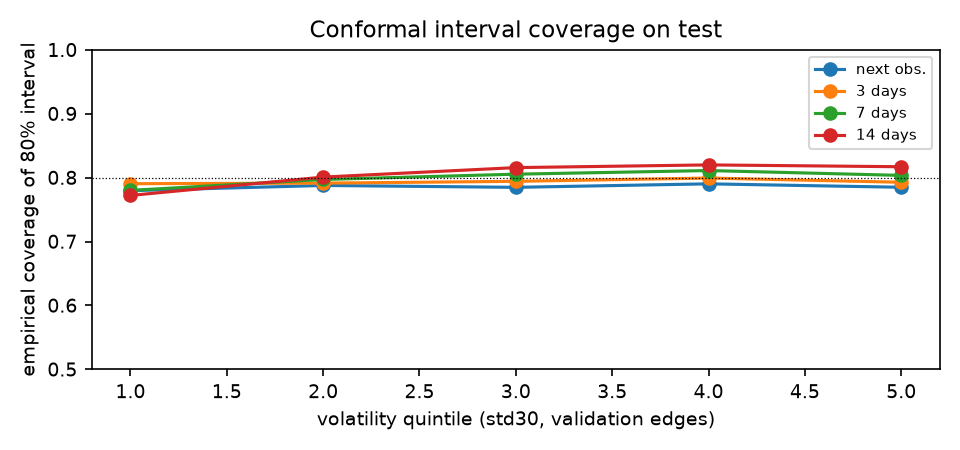
\includegraphics[width=0.72\linewidth]{interval_coverage.png}
\caption{Historical test coverage of 80\% split-conformal intervals by volatility quintile (bin edges from validation).}\label{fig:cov}
\end{figure}

\paragraph{Provenance effect.}
Measured on the mirror after the November 2025 portal change:
\begin{itemize}
  \item 80\% coverage fell to 67.6--72.9\%;
  \item relative MAE weakened to 0.993, 0.977, 0.968 and 0.944.
\end{itemize}
This had the hallmarks of a distribution shift.
Re-scoring the \emph{same frozen models} on the complete official record for the same period (Table~\ref{tab:prov}) gives:
\begin{itemize}
  \item coverage of 78.0--78.7\%, a loss of only 1.2--2.2 points against the pre-change period;
  \item relative MAE of 0.976, 0.962, 0.962 and 0.937.
\end{itemize}
The two record sets differ in which rows exist: after the change the mirror has only 62,845--97,079 test rows per horizon, against 332,275--391,425 officially.
We therefore also score both on the identical (series, origin) keys present in both (50,923--78,773 rows per horizon; last block of Table~\ref{tab:prov}).
On these identical rows, mirror coverage is 68.0--72.3\% and official coverage 78.8--79.7\%. The calibration loss is therefore not an artefact of sample composition.
The contrast is consistent with source incompleteness affecting the evaluation; the matched-origin comparison does not isolate which changed features or target reports contribute how much.
Accuracy is a different matter. On official data the 7-day relative MAE still rises from 0.938 before the change to 0.962 after, so the gain over persistence shrinks from 6.2\% to 3.8\%. A smaller accuracy shift remains on the official source.
The mechanism is consistent with Section~\ref{sec:data}: three-times-longer gaps make ``next'' targets more distant and trailing windows sparser, so realised changes exceed what validation residuals calibrated on denser series anticipate.
A provenance audit is therefore a precondition for any claim about drift in this data.

\begin{table}[t]\centering\small
\caption{Frozen models after the November 2025 portal change (2025-11-01 to 2026-04-20): mirror versus complete official record.}\label{tab:prov}
\begin{tabular}{@{}lrrrr@{}}\toprule
 & next & 3 d & 7 d & 14 d\\\midrule
Rel.\ MAE, mirror & 0.993 & 0.977 & 0.968 & 0.944\\
Rel.\ MAE, official & 0.976 & 0.962 & 0.962 & 0.937\\
80\% coverage, mirror & 67.6\% & 71.3\% & 72.0\% & 72.9\%\\
80\% coverage, official & 78.0\% & 78.7\% & 78.7\% & 78.5\%\\\midrule
\multicolumn{5}{@{}l}{\emph{Identical (series, origin) keys}}\\
Rel.\ MAE, mirror & 0.998 & 0.983 & 0.971 & 0.942\\
Rel.\ MAE, official & 0.972 & 0.958 & 0.959 & 0.930\\
80\% coverage, mirror & 68.0\% & 71.6\% & 71.9\% & 72.3\%\\
80\% coverage, official & 78.8\% & 79.7\% & 79.7\% & 79.3\%\\\bottomrule
\end{tabular}\end{table}

\section{Later-period evaluation and retraining}\label{sec:prospective}

\paragraph{Frozen models on later data.}
The models, conformal quantiles and MASE scales of the main experiment were saved on 2026-10-22. The official back-fill that first brought reports after 2026-04-21 into the project ran on 2026-10-23.
The saved models were scored, without refitting, on official reports for 2026-04-22 to 2026-10-22.
This is a post-development hold-out rather than a real-time evaluation: the reports existed when the models were saved, but no development step had access to them.
The scope is the same panel of series, with 0.27--0.31 million forecasts per horizon.
Table~\ref{tab:prosp} shows the results. The relative MAE is 0.963, 0.955, 0.958 and 0.952, and the DM tests reject equal accuracy with persistence at every horizon ($p<2\times10^{-15}$).
The 80\% intervals cover 76.9--80.1\%.
At 7 and 14 days the gain is smaller than in the main test (0.958 against 0.938 at 7 days), The evaluated refit did not recover the earlier gain (Table~\ref{tab:retrain}); this comparison alone cannot attribute the difference to model age or market conditions.

\begin{table}[t]\centering\small\setlength{\tabcolsep}{4pt}
\caption{Frozen models (trained up to 2023), with relative MAE and 80\% coverage. The first block re-scores the main test period on the complete official record. The second is post-development retrospective scoring (2026-04-22 to 2026-10-22).}\label{tab:prosp}
\begin{tabular}{@{}lrrrr@{}}\toprule
 & next & 3 d & 7 d & 14 d\\\midrule
Rel.\ MAE, main test (official) & 0.972 & 0.954 & 0.943 & 0.925\\
80\% coverage, main test (official) & 79.2\% & 79.6\% & 80.0\% & 80.3\%\\
Rel.\ MAE, later-period & 0.963 & 0.955 & 0.958 & 0.952\\
80\% coverage, later-period & 76.9\% & 78.8\% & 79.6\% & 80.1\%\\
Series better than persistence, later-period$^a$ & 59.3\% & 64.1\% & 66.6\% & 66.0\%\\\bottomrule
\end{tabular}
\par\smallskip\footnotesize $^a$ Among 2,497--2,701 series with at least 30 later-period rows (about 8,600 in the main test).\end{table}

\paragraph{Does retraining help?}
We retrained under the protocol fixed in Section~\ref{sec:protocol}: training up to 2024, validation on 2025, and a final test from 2026-01-01 to 2026-10-22 that was not used for any retraining choice.
The search space, selection rule, sample size and features were the same as before.
Validation selected absolute-loss boosting at the next report and at 3 days, the random forest at 7 days and squared-loss boosting at 14 days.
Table~\ref{tab:retrain} compares the retrained and frozen models on identical final-test rows.
No difference is significant (DM $p$ between 0.12 and 0.99). The retrained model is numerically worse at 14 days (0.950 against 0.946).
Both models beat persistence at every horizon ($p\le1.4\times10^{-12}$). The moving-average, seasonal-naive and seasonal-adjusted baselines are again worse than persistence (relative MAE 1.007--3.98).

\begin{table}[t]\centering\small\setlength{\tabcolsep}{4pt}
\caption{Final test, 2026-01-01 to 2026-10-22, with identical rows for both models. The DM test compares the retrained model with the frozen one.}\label{tab:retrain}
\begin{tabular}{@{}lrrrrr@{}}\toprule
Horizon & Test rows & Rel.\ MAE, frozen & Rel.\ MAE, retrained & DM $p$ & 80\% coverage (frozen / retrained)\\\midrule
next & \num{553801} & 0.965 & 0.966 & 0.12 & 77.0\% / 77.5\%\\
3 d & \num{531321} & 0.955 & 0.955 & 0.99 & 78.6\% / 78.8\%\\
7 d & \num{519251} & 0.958 & 0.958 & 0.74 & 79.3\% / 78.9\%\\
14 d & \num{496306} & 0.946 & 0.950 & 0.35 & 79.7\% / 78.1\%\\\bottomrule
\end{tabular}\end{table}

\paragraph{Exploratory operational adoption of LightGBM.}
Before that candidate training run, we committed an operational rule for replacing the served model; the evaluation period had already been examined, so this was not confirmatory pre-registration. The candidate had to beat the frozen model at 7 days after a Holm correction, be significantly worse at no horizon, and keep 80\% coverage within 75--85\%, losing no more than two points relative to the frozen model. Its published forecasts also had to reproduce its offline predictions exactly.
A LightGBM candidate trained under the retraining protocol (validation used only for the number of leaves, early stopping and calibration) reached relative MAE 0.944, 0.933, 0.934 and 0.922 on the rows of Table~\ref{tab:retrain}. It was better than both Spark models at every horizon (Holm-adjusted $p\le4\times10^{-16}$), with 80\% coverage of 77.5--79.0\%. It was adopted for the prototype on this exploratory evidence.
Because this final period had already been used twice, and an earlier LightGBM result on overlapping data had motivated the test, neither the adoption nor subsequent cleaning sensitivity independently confirms LightGBM superiority. The later smaller-model experiments compare LightGBM with simple baselines, not with newly refitted Spark alternatives.

\paragraph{Interpretation and disclosure.}
Two more years of data did not measurably improve this model class on 2026.
This is a single refit on one final period. It does not show that retraining never helps, and it does not make the frozen models current: they encode no information after 2023.
The final test is not pristine. January to April 2026 belonged to the main test, and April to October 2026 had already been used to score the frozen models (above), before the retraining protocol was fixed. No choice in the retraining run used any 2026 data.

\paragraph{Separate-calibration and cleaning sensitivity.}
The locked smaller-model experiment in Section~\ref{sec:protocol} completed on clean fitting-source commit \texttt{e7abad9}; reporting code \texttt{059e8e2} recomputes aggregate metrics and statistical summaries from checksum-verified predictions. The unfiltered feature fingerprint was captured after the build: it supports subsequent integrity checks but does not prove the exact executed builder and input state at build time. Original cleaned-feature construction likewise remains incompletely attributed.
Table~\ref{tab:revision} reports the results. Candidate MAE on cleaned rows rises from INR 192.30 at the next report to INR 393.83 at 14 days, compared with persistence MAE of INR 202.26 and INR 411.51. Unfiltered values are INR 197.04 and INR 397.39, against INR 207.30 and INR 416.21. All other simple baselines are worse than persistence in each regime (relative MAE 1.001--3.980). Holm-adjusted p values for the eight candidate--persistence comparisons are below $5\times10^{-23}$, but their small values do not establish practical value for individual farmers.

\begin{table}[t]\centering\small\setlength{\tabcolsep}{4pt}
\caption{Retrospective robustness with disjoint selection and calibration periods. MASE columns show candidate/persistence. Confidence intervals are paired 28-calendar-day block bootstrap intervals for relative MAE (500 replicates), conditional on fitted models.}\label{tab:revision}
\begin{tabular}{@{}llrrrr@{}}\toprule
Regime & Horizon & Rel. MAE & MASE & Coverage 80\% & Rel. MAE 95\% interval\\\midrule
cleaned & next & 0.951 & 1.10/1.16 & 77.7\% & [0.946, 0.955] \\
cleaned & h3 & 0.943 & 1.00/1.06 & 79.0\% & [0.939, 0.947] \\
cleaned & h7 & 0.952 & 1.07/1.11 & 79.5\% & [0.949, 0.956] \\
cleaned & h14 & 0.957 & 1.04/1.06 & 79.4\% & [0.953, 0.962] \\
unfiltered & next & 0.951 & 1.11/1.17 & 77.8\% & [0.945, 0.955] \\
unfiltered & h3 & 0.941 & 1.01/1.07 & 79.1\% & [0.936, 0.946] \\
unfiltered & h7 & 0.950 & 1.08/1.12 & 79.5\% & [0.946, 0.954] \\
unfiltered & h14 & 0.955 & 1.05/1.06 & 79.5\% & [0.949, 0.960] \\
\bottomrule\end{tabular}

\end{table}

MASE exceeds one in every regime/horizon, despite gains against contemporaneous persistence: the training-period scale and current-period persistence error are different denominators. Intervals under-cover most noticeably at the next report (77.7--77.8\%). Across the eight fits, monthly relative MAE ranges from 0.931 to 0.972; 60.6--68.5\% of entities have lower aggregate candidate error. Separate entity-cluster confidence intervals also lie below one; these do not combine temporal and cross-sectional uncertainty into a two-way guarantee. Full baselines, 14-day-block estimates, monthly values, interval widths and cluster estimates are retained in the reproducible result tables.
On common origins, cleaned/unfiltered relative MAE is 0.951/0.952, 0.943/0.944, 0.952/0.951 and 0.957/0.956. The direction of the gain therefore survives this sensitivity, but its magnitude is pipeline-dependent; targets and features may differ even on common origins. Of 14,098,524 valid reports in the unfiltered build scope, 18,775 trigger the jump flag. Inspection of 120 deterministically selected reports cannot distinguish reporting errors from genuine economic shocks and supplies no manual ground truth.
No serving model was changed by this study. A genuine confirmation must archive forecasts before their outcomes and remains future work.

\section{Decision-rule back-test, discussion and limitations}\label{sec:discussion}

\paragraph{Decision rule.}
The application maps the 7-day 80\% interval $[\ell_7,u_7]$ (on the log-return scale) to cautious market-outlook cards. Holding cost is $c=1\%+$ 5\%/week for perishables (1\%/week for durables); these costs are placeholders that the farmer can edit.
\begin{itemize}
  \item \textsc{hold} if $\ell_7\ge\ln(1+c)$;
  \item \textsc{sell} if $u_7\le0$;
  \item \textsc{compare} if a market in the same state reported a price at least 5\% higher within three days, before transport costs (which the farmer enters; the default is zero);
  \item \textsc{watch} otherwise.
\end{itemize}
On the main test the rule (configuration version 2026-10-22.1) abstains on 98.5\% of report-days.
\textsc{hold} fires on 0.5\%, and the realised price exceeds today's plus cost 80.0\% of the time. \textsc{sell} fires on 1.0\%, with a hit rate of 67.8\%.
\textsc{hold} fires mostly after reports far below a series' recent level that then revert (median realised change $+46.8\%$). Some of these may be reporting errors below the sanity threshold.
These are hit rates on published modal prices, not farm-gate profits, and \textsc{compare} is not back-tested because transport costs are unknown.

\paragraph{Comparison with published results.}
Published mandi studies use different markets, horizons, aggregation and splits. Their MAPE values (e.g.\ \cite{manogna2025deep}) are not comparable with our WAPE.
The historical comparisons are internal and exploratory; they are not independently confirmed by the smaller release study:
\begin{itemize}
  \item learned models beat persistence by 3--8\%;
  \item they match a per-series smoother at 1--3 days;
  \item cross-market features account for 17--29\% of the 7-day gain, depending on the learner;
  \item a global LightGBM beats the MLlib model by a further 0.023--0.031 in relative MAE.
\end{itemize}
These effects are far smaller than gains over ARIMA reported elsewhere, which suggests that baselines and protocol may explain much of the spread in reported accuracy.

\paragraph{Threats to validity.}
\begin{itemize}
  \item Model choice, conformal calibration and the panel definition use pre-test data, but the conformal quantiles are calibrated on the same validation year used for selection.
  \item For backtest folds within 2021--2023, the panel was selected on reporting density in those years. No prices enter this density rule, but later reporting availability still influences early-fold membership.
  \item Original Diebold--Mariano tests treat daily cross-sectional mean losses as one series. We report one test per model and horizon against persistence without a multiplicity correction; these p values are descriptive historical results, not the corrected primary family of the separate robustness experiment; a historical sensitivity at Newey--West lag 20 also gave small heuristic p values ($p\le8\times10^{-13}$ at every horizon).
  \item Forecast rows are not independent statistical replicates. The temporal unit is the aggregated calendar day; even those days are correlated. Limited seasons, panel changes and common shocks constrain inference. Holm correction cannot repair misspecified dependence or exploratory selection.
  \item The automated independent statistical-method review is not human expert sign-off; submission requires that additional review.
  \item Results describe well-reported mandis of 36 commodities.
  \item Modal price is the published summary, not an individual farmer's price.
\end{itemize}

\paragraph{Limitations.}
\begin{itemize}
  \item The MLlib search space is small (8 configurations per horizon), and the LightGBM model now in service was adopted on a final period that had already been used twice (Section~\ref{sec:prospective}).
  \item Only one retraining was evaluated (Section~\ref{sec:prospective}).
  \item No deep or foundation-model baselines were run.
  \item Arrivals and weather covariates are absent.
  \item Adaptive conformal methods were not implemented.
  \item A validated refresh job exists, but no schedule is installed. Freshness therefore depends on operator runs.
\end{itemize}

\paragraph{Ethics.}
Forecasts can hurt farmers who over-trust them. The interface therefore:
\begin{itemize}
  \item shows intervals, measured error and data age;
  \item defaults to \textsc{watch};
  \item never states a guaranteed price.
\end{itemize}
No personal data is collected. Interface translations into five Indian languages are machine-drafted and await native-speaker review. Welfare effects are not claimed \cite{fafchamps2012sms,mitra2018asymmetric}.

\bibliographystyle{plainnat}
\bibliography{references}
\end{document}
